\chapter{Einleitung}

\section{Problemstellung}
Code Quality ist ein oft unterschätzter Teil der Softwareentwicklung. Viele Bugs und Sicherheitslücken können durch eine gesteigerte Code Quality vermieden werden. Um die Code Quality in einem Software-Projekt zu verbessern, werden Hilfsmittel eingesetzt, wie Tools für die Statische Code Analyse. Eine Statische Code Analyse überprüft den Code während der Übersetzungszeit (Compiler Übersetzung) und zeigt auftretende Fehler sowie verschiedene Warnungen auf. Für die Anzeige der Ergebnisse der Statischen Code Analyse gibt es verschiedene Möglichkeiten: Direkte Anzeige in der Entwicklungsumgebung, Anzeige in einer eigenen (Web-)Applikation oder in einer Ausgabe als Report. Die daraus folgenden Informationen sind aber rudimentär, d.h. text-basiert und unübersichtlich (siehe Abbildung \ref{fig:findingsInIDE}). Ebenso wird eine Verbesserung des Codestils nur schwer erreicht, da die Informationen nicht dauerhaft verfügbar sind. Die Analysen gestalten sich daher nur als Momentaufnahme aus dem Code. 

\begin{figure}[tp]
  \centering
  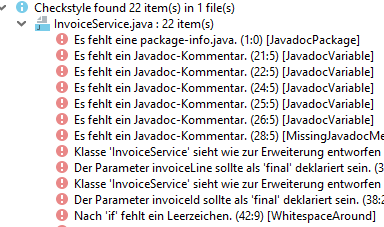
\includegraphics[height=5cm]{images/ideChecks.PNG}
  % The short caption should be capitalised
  % The full caption should hold a full sentence. 
 \caption[Anzeige von Fehler in der Entwicklungsumgebung Intellij IDEA]{Anzeige von Fehler in der Entwicklungsumgebung Intellij IDEA.}
  \label{fig:findingsInIDE}
\end{figure}

Ein Problem bei Applikationen, die am Desktop oder am Server installiert werden können, ist auch die fehlende Individualität, da die eingesetzten Tools  und Techniken nicht selbst angegeben werden können. Hingegen muss die vorgegebene Code Analyse-Technik verwendet werden. Das Problem dabei ist, dass einzelne Tools für bestimmte Probleme und Einsatzgebiete besser geeignet sind.

\section{Zielsetzung und Forschungsfragen}

Dadurch stellt sich die Frage, wie mit den Daten der Statischen Code Analyse weiterreichende Analysen und dauerhafte Informationsübersichten erstellt werden können und welche Möglichkeiten es gibt, daraus einen langfristigen Vorteil für die Entwicklerin oder den Entwickler zu erreichen. Das Ziel ist es daher, verschiedene Analyse- und Aufbereitungsmöglichkeiten der Daten zu entwickeln, die der Benutzerin oder den Benutzer bei der Verbesserung in der Entwicklung unterstützen und dadurch die Code Qualität in Projekten langfristig zu erhöhen.

\subsection{Methodik} 

Mithilfe einer Webapplikation werden Daten verschiedener Code-Analyse-Tools ausgewertet und präsentiert. Dazu werden in mehreren verschiedenen Projekten diese Tools eingesetzt. Die Analysen in der Webapplikation bauen auf diese Daten auf, die mithilfe eines Plugins oder eines Datenbank-Imports gespeichert werden. Die Präsentation und Visualisierungen sollen unabhängig von den eingesetzten Tools sein.

Um die Effizienz, Einfachheit bei der Anwendung, Mehrwertigkeit und Unterstützungshilfe der Webapplikation und der Analysen festzustellen, werden Tests und Anwendungsfälle mit verschiedenen Entwicklerinnen und Entwicklern durchgeführt. Die durchführenden Benutzerinnen und Benutzer sollen hierbei einen unterschiedlichen Wissenstand im Bereich der Softwareentwicklung aufweisen, sodass die Ergebnisse nur auf der Webapplikation und nicht auf Wissen über bestimmte Tools und Fehler basieren. 


Beim Durchführen der Tests muss darauf geachtet werden, dass sich das Testsetup und die Testumgebung nicht unterscheidet. Die Ergebnisse der Tests werden protokolliert. Im Test können die Testpersonen mit der Applikation direkt und interaktiv arbeiten. Dies geschieht im Rahmen eines Interviews, wo die Anwenderinnen und Anwender Erfahrungen mit der Applikation, Kritikpunkte und Vorschläge einbringen können. Der Test beginnt mit einer zurückgesetzten Datenbank und einem leeren Frontend. Mittels einer Bildschirmübertragung, bei der die Testpersonen auch die Steuerung des Computers übernehmen können, wird der Test durchgeführt.
Der Test beinhaltet die Beantwortung von vorgefertigten Fragen, das Ausführen der Funktionen, das Suchen von angezeigten Fehlern sowie offenes Feedback.
Die Tests finden online statt haben einen Zeitrahmen von 30 bis 45 Minuten. 
\subsection{Kriterien} 
Testpersonen evaluieren die Arbeit anhand folgender Kriterien und Punkte:
\begin{itemize}
\item Einfachheit \\ Die Verwendung der Applikation soll unkompliziert und einfach geschehen. Dies beinhaltet den Einbau des Plugins, das Starten der Applikation und die Auswahl der richtigen Daten.
\item Übersicht \\ Im Frontend sollen alle wichtigen Informationen übersichtlich und gut lesbar aufbereitet werden. Ebenso kann der Benutzer bestimmte Daten selektieren, um einen genaueren Überblick zu bekommen.
\item Unterstützungshilfe \\ Durch die Visualisierungen, Tabellen und andere Funktionalitäten soll der Benutzer eine kurz und langfristige Unterstützung bei der Entwicklung bekommen.
\item Individualität \\ Die Applikation soll für die Arbeit der Benutzerinnen und Benutzer und deren eingesetzten Code Analyse Tools verfügbar und kompatibel sein. 
\item Performance \\ Die Benutzerin oder der Benutzer kann nach einsetzen der Applikation schnell seine Daten einsehen.
\item Verständlichkeit \\ Die Visualisierungen und Funktionalitäten sollen für die Benutzerinnen und Benutzer ohne Hilfestellungen verständlich sein und sollen daher ohne Probleme verwendet und angewandt werden können.
\end{itemize}

Ebenso werden anhand dieser Kriterien die Unterschiede zu herkömmlichen Lösungen erarbeitet. Die Arbeit ist erfolgreich, wenn diese Kriterien zutreffen. 

